\documentclass[aspectratio=169]{beamer}

\usepackage[utf8]{inputenc}
\usepackage{array}
\usepackage{booktabs}
\usepackage{bold-extra}
\usepackage{graphics}
\usepackage{hyperref}
\hypersetup{%
  colorlinks=true,
  linkcolor=blue,
  filecolor=blue,
  urlcolor=cyan,
}
\usepackage{multicol}
\usepackage{setspace}
\usepackage{verbatim}
\usepackage{fancyvrb} % for verbatim centering

\usetheme{Warsaw}
\usecolortheme{beaver}
\definecolor{clOrange}{HTML}{E76600}
\definecolor{clAlmostWhite}{HTML}{FEFFD9}
\definecolor{clGreen}{HTML}{007F00}
\definecolor{clFlag}{HTML}{D33682}
\definecolor{clFlagOpt}{HTML}{CB4B16}
\definecolor{clRedFlag}{HTML}{DC322F}
\definecolor{clViolet}{HTML}{4c0070}

\title[LTN04 :: Cpp20\_Modules]{C++20 feature: Modules}
\author{Adam Graliński}
\date[FFFE\_21]{\textbf{C++ {\color{red}F}{\color{blue}F}{\color{green}F}{\color{yellow}E}, April 2021}}

\setbeamertemplate{navigation symbols}{}
\setbeamercolor{title}{fg=black}
\setbeamercolor{author}{fg=clAlmostWhite}
\setbeamercolor{date}{fg=clAlmostWhite}
\setbeamerfont{author}{size=\huge}
\setbeamerfont{date}{size=\Large}

\begin{document}

{\usebackgroundtemplate{%
 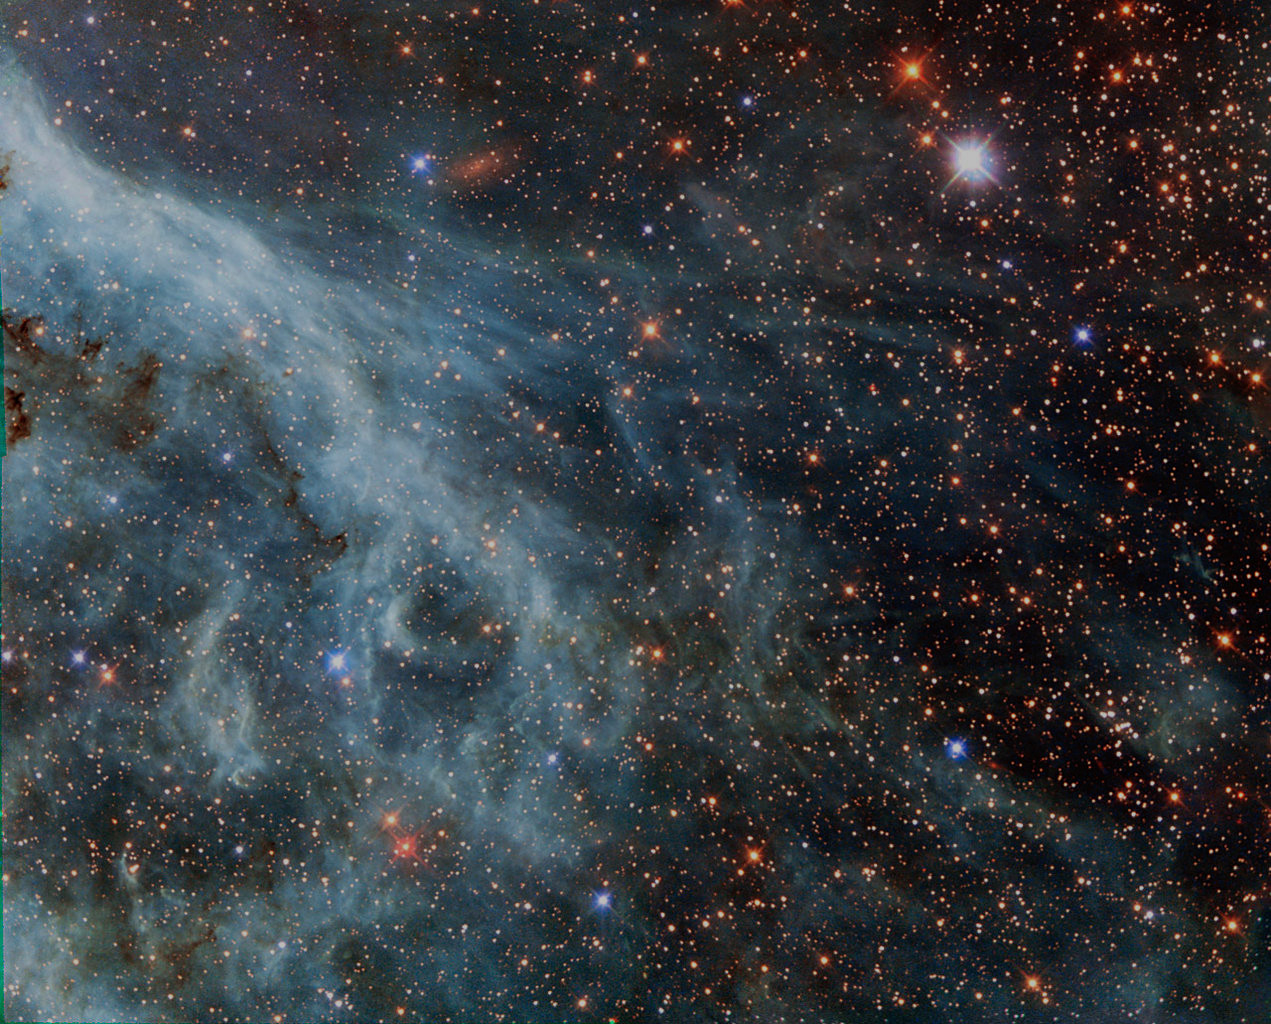
\includegraphics[width=\paperwidth,height=\paperheight]{../common/bg_galaxy.jpg}}
\begin{frame}
\titlepage{}
\end{frame}
}

\begin{frame}
\frametitle{Why modules?}
\Large{\textbf{\textcolor{clViolet}{Pay only for what is being used}} approach is \textbf{awesome}}
\begin{itemize}
  \item{holds for runtime}
  \item{kind of does not hold for compilation time}
  \begin{itemize}
    \item{long headers with lots of template instantiating}
    \begin{itemize}
      \item{such as Boost}
      \item{such as STL}
    \end{itemize}
  \end{itemize}
\end{itemize}
\end{frame}

\begin{frame}
\frametitle{Why modules?}
Problem: \textcolor{clViolet}{Long compilation time penalty}
\linebreak{}
Solution:
\begin{table}
  \begin{tabular}{l l l l}
    \textit{version} \hspace{1cm} &
    \textit{solution} \hspace{1cm} &
    \textit{pros} &
    \textit{cons} \\
    \midrule{}
    C++17 & \textbf{precompiled} & some* & lots* \\
    and before & \textbf{headers} & & \\
    \midrule{}
    C++20 & \textbf{\textcolor{violet}{modules}} & lots & still not widely supported \\
  \end{tabular}
\end{table}
\end{frame}

\begin{frame}[fragile]
\frametitle{How to use?}
{\Large \href{https://en.cppreference.com/w/cpp/language/modules}
             {https://en.cppreference.com/w/cpp/language/modules}}
\vspace{1ex}
{\scriptsize
\begin{verbatim}
// helloworld.cpp
export module helloworld;  // module declaration
import <iostream>;         // import declaration

export void hello() {      // export declaration
    std::cout << "Hello world!\n";
}
\end{verbatim}

\begin{verbatim}
// main.cpp
import helloworld;  // import declaration

int main() {
    hello();
}
\end{verbatim}
}
\end{frame}


\begin{frame}
\frametitle{Compiler support}
{\Large You'll need a modern compiler with support for modules.} \linebreak{}
{\small (note: at the time of writing this, modules support is partial/incomplete for every existing compiler. However, it is complete enough to compile the example code.)}
\vspace{1ex}
\begin{itemize}
  \item{\texttt{-std=c++20} or \texttt{-std=c++2a}}
  \item{\textbf{clang}: works out of the box since 11.0. See
  \href{http://www.open-std.org/jtc1/sc22/wg21/docs/papers/2019/p1766r1.html}{P1766R1}.}
  \item{\textbf{gcc}: works.}
  \begin{itemize}
    \item{P1766R1 is \textbf{\textcolor{clRedFlag}{not}} supported, but many others are}
    \item{requires g++ version 11}
    \item{requires extra flag: \texttt{\textcolor{clFlag}{-fmodules-ts}}}
  \end{itemize}

  \item{\textbf{MSVC}: basic support is claimed}
  \begin{itemize}
    \item{VS 2019 with Modules (16.8 preview 3) or later required}
    \item{I was unable to verify this :-)}
  \end{itemize}

\end{itemize}
\end{frame}


\begin{frame}[fragile]
\frametitle{How to compile?}
  \begin{enumerate}
    \item{Precompile the module code to binary module interface}
    \begin{verbatim}
clang++ -std=c++2a -c helloworld.cpp -Xclang
        -emit-module-interface -o helloworld.pcm
    \end{verbatim}

    \item{Compile c++ sources and link them}
    \begin{verbatim}
clang++ -std=c++2a -fprebuilt-module-path=. main.cpp helloworld.cpp
    \end{verbatim}
  \end{enumerate}

  {\footnotesize Taken from Arthur O'Dwyer 's excellent
  \href{https://quuxplusone.github.io/blog/2019/11/07/modular-hello-world/}
  {article}.}
\end{frame}


\begin{frame}[fragile]
\frametitle{Granular control over exports}
\begin{verbatim}
export module MyModule;
void Foo() { /* do important stuff */ }
export void Bar() {
  Foo();
}
\end{verbatim}

\begin{verbatim}
import MyModule;

int main() {
  Bar(); // OK
  // Foo(); // won't compile!
}
\end{verbatim}
\end{frame}

\begin{frame}[fragile]
\frametitle{What next?}
{\Large \href{https://eel.is/c++draft/module}{https://eel.is/c++draft/module}}
\\
{\Large \href{https://blog.ecosta.dev/en/tech/explaining-cpp20-modules}
{https://blog.ecosta.dev/en/tech/explaining-cpp20-modules}}
\\
\vspace{2ex}
\center {\Large Thank you!}

\end{frame}
\end{document}
